\documentclass[11pt]{article}
\usepackage{amsmath}
%\usepackage{extsizes}
\usepackage{amsmath,amssymb}
%\usepackage{omegavn,ocmrvn}
%\usepackage[utf8x]{inputenc}
\usepackage[utf8]{vietnam}

\usepackage{listings}
\lstset{language=Matlab}          % Set your language (you can change the language for each code-block optionally)


\usepackage{longtable}
\usepackage{answers}
\usepackage{graphicx}
\usepackage{array}
\usepackage{pifont}
\usepackage{picinpar}
\usepackage{enumerate}
\usepackage[top=3.0cm, bottom=3.5cm, left=3.5cm, right=2.5cm] {geometry}

\usepackage{extarrows}
\usepackage{hyperref}


\newtheorem{bt}{Câu}
\newcommand{\RR}{\mathbb R}
\Newassociation{sol}{Solution}{ans}
\newtheorem{ex}{Câu}
\renewcommand{\solutionstyle}[1]{\textbf{ #1}.}


\begin{document}
% \noindent

\begin{tabular*}
	{\linewidth}{c>{\centering\hspace{0pt}} p{.5\textwidth}}
	ĐẠI HỌC QUỐC GIA HÀ NỘI	
	 & {ĐỀ THI KẾT THÚC HỌC PHẦN}  
	\tabularnewline
	TRƯỜNG ĐẠI HỌC KHOA HỌC TỰ NHIÊN & {HỌC KỲ II, NĂM HỌC 2021-2022}
	% Exercises on pages 239, 240 Cheney/Kincaid are really nice
	\tabularnewline
	\rule{3in}{1pt}  \small  & \rule{2in}{1pt} %(Due date:)
	\tabularnewline
	%  \tabularnewline
	%  &(Đề thi có 1 trang)
\end{tabular*}

\def\hro{\mathbb}
\def\vphi{\varphi}
\def\tet{\theta}
\def\a{\alpha}
\def\b{\beta}
\def\rar{\rightarrow}
\def\R{\hro{R}}
\def\C{\hro{C}}
\def\Si{\Sigma}
\def\si{\sigma}
\def\ep{\varepsilon}
\def\rank{\mathrm{rank}}
\newcommand{\m}[1]{
	\begin{bmatrix}
		#1
	\end{bmatrix}
}


\begin{center}
Tên học phần: {\bf Thực Hành Tính Toán Khoa Học} \\ 
Mã học phần: \textbf{MAT3525}	\quad Số tín chỉ: \textbf{03} \quad	Đề số: \textbf{01} \\ 
% Dành cho sinh viên lớp học phần: MAT3525 \\
%Thời gian làm bài: \textbf{90 phút} (không kể thời gian phát đề) \quad Đề bao gồm: \textbf{02 trang}
\end{center}

\begin{bt}
Toàn bộ các bài trong Mục 2.4 này các em làm chung vào 1 file Problem1.m \\
%	
\begin{figure}[h!]
	\centering
	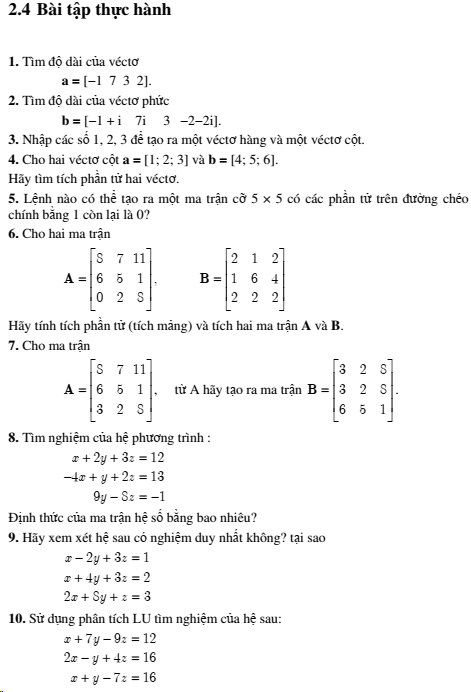
\includegraphics[width=0.65\linewidth]{K65_1}
	\caption{Trang 51 sách Nguyễn Quang Hoàng pdf}
	\label{fig:k651}
\end{figure}
\end{bt}

\newpage 

\begin{bt}\label{Problem 2}
Toàn bộ các bài trong Mục 3.5 này các em để chung vào 1 folder Problem2. \\
%	
\begin{figure}[h!]
	\centering
	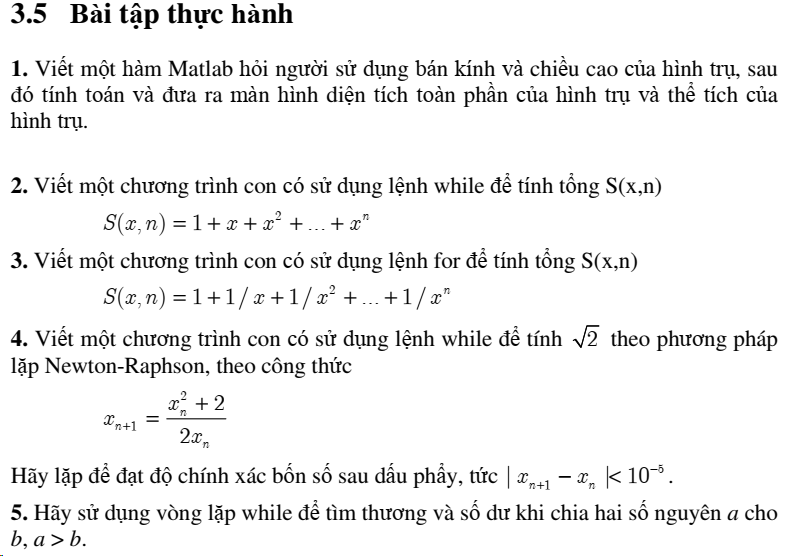
\includegraphics[width=0.75\linewidth]{K65_2}
	\caption{Trang 71 sách Nguyễn Quang Hoàng pdf}
	\label{fig:k652}
\end{figure}
\end{bt}


\begin{bt}\label{Problem 3}
Toàn bộ các bài trong Mục 4.3 này các em để chung vào 1 folder Problem3. \\
%	
\begin{figure}[h!]
	\centering
	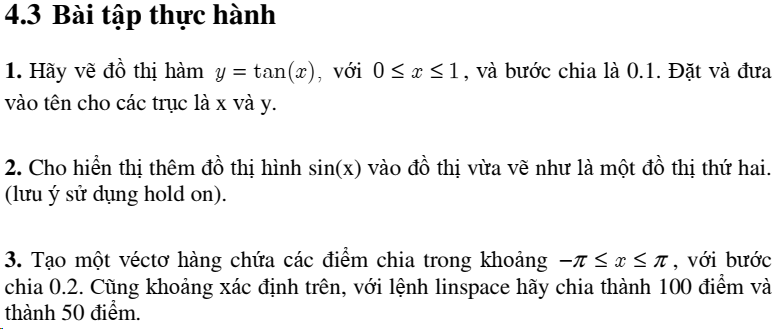
\includegraphics[width=0.75\linewidth]{K65_3}
	\caption{Trang 113 sách Nguyễn Quang Hoàng pdf}
	\label{fig:k653}
\end{figure}
\end{bt}

\newpage 

\begin{bt}
Đọc trước về cách sử dụng ode23 và ode45 trong Chương 6 để giải các bài tập sau. Có thể viết gộp các bài vào chung 1 file bằng cách sử dụng cú pháp switch (trang 66 bản pdf) trong MATLAB.\\
%	
\begin{figure}[h!]
	\centering
	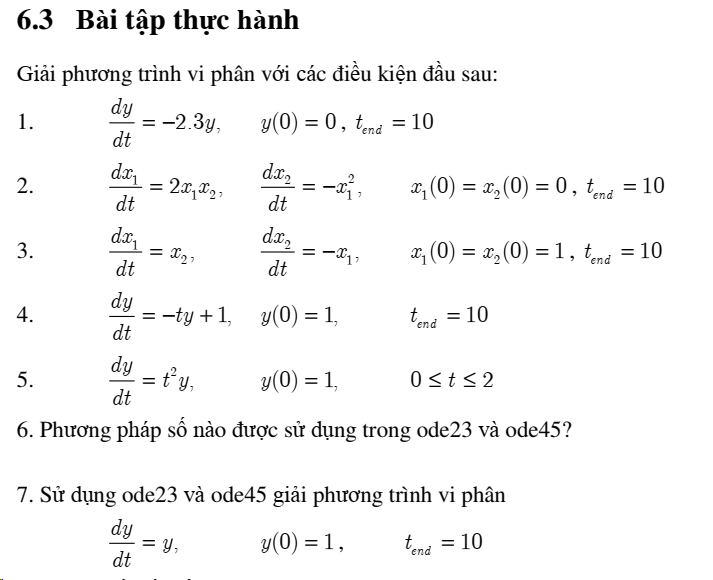
\includegraphics[width=0.75\linewidth]{K65_4}
	\caption{Trang 139 sách Nguyễn Quang Hoàng pdf}
	\label{fig:k654}
\end{figure}
%
\end{bt}

\end{document}



